\chapter{研究现状和相关工作}

\section{本章引言}

本章首先介绍了影视剧产业在社交网络上的发展与应用,包括利用社交网络数据对影视剧的票房进行预测,针对观众喜欢为其进行影视剧推荐。由于在社交网络上对影视剧进行宣传推广时,需要在众多的推广方式当中选取推广效果最好的方式,因此需要分析各种推广方式与推广结果之间的因果关系,本章主要对工具变量法、断点回归设计、格兰杰因果关系检验这三种因果分析方法进行了介绍,简要介绍了其分析原理以及现阶段的应用情况。最后针对演员在微博上推广电视剧的行为特点,本章选取倾向值匹配算法作为因果分析方法,并对其进行了介绍。

\section{影视剧与社交网络}

影视剧属于传统产业,诞生与发展由来已久,而社交网络属于新兴事物,近几年才蓬勃发展起来。但是随着社交网络的不断进步,影视剧与社交网络的结合越来越紧密,人们发现利用社交网络对影视剧的制作、宣传都能够起到积极作用。目前在社交网络领域关于影视剧的研究主要集中在两个方面,一是利用社交网络数据对影视剧进行预测,二是针对影视剧的推荐。

利用社交网络数据对影视剧进行预测,主要集中在大数据和机器学习领域。由于网络数据量的日益增大,通过大数据分析其内在关系,利用机器学习找出其中的统计学关系,更好地指导、预测影视剧的发展。其中最典型的应用之一即为票房预测,通过挖掘社交网络当中影视剧的相关信息,来预测未来影视剧票房收视率的发展趋势。例如王伟在文献\cite{王伟2015基于微博数据的电影票房预测研究}中利用多元线性回归模型、BP神经网络模型、支持向量机模型等预测模型,对微博上关于电影的微博数量、情感、营销等特征进行分析,预测电影票房情况。王晓耘等人在文献\cite{王晓耘2016基于微博的电影首映周票房预测建模}中对关于影视剧微博的情感倾向进行了分析,通过SVM算法对其进行分类,识别出观众观看意愿的强烈程度,再利用BP神经网络模型进行票房预测,能够准确地预测出电影上映首周的票房情况。王烁等人在文献\cite{王炼2014基于网络搜索的票房预测模型}中分析了网络搜索量与电影票房之间存在的联系,由于大多数观众习惯在观影之前通过网络搜索相关评论来确定是否要购票观看,因此,网络搜索量与票房之间也就存在一定的正相关关系,通过最小二乘法等方法可以通过搜索量的变化预测电影票房的变化。

\begin{figure}[h] 
  \centering
  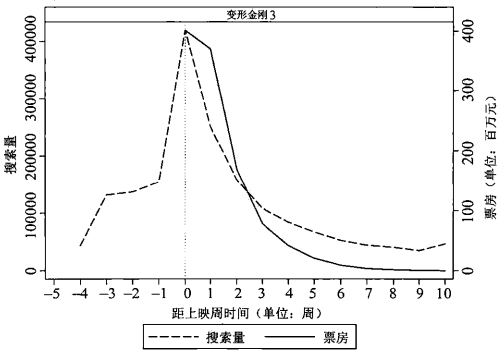
\includegraphics[height=8cm]{票房}
  \caption{网络搜索量与票房之间的关系}
\end{figure}

同样,国外学者在票房预测领域也有着深入的研究。Sharda等人在文献\cite{sharda2006predicting}中将影视剧的票房预测问题转化为了票房收益的分类问题,避免预测具体收益值而是转为预测收益区间,这样的预测结果更加准确合理,能够为各层次用户提供参考依据。作者通过神经网络模型进行预测,并与其它算法进行了10倍交叉验证比较,证明其取得了更好的预测效果。

Asur等人在文献\cite{asur2010predicting}中利用社交网站Twitter上关于电影的评论来预测票房。作者通过收集评论信息并对其进行情感分类,通过分析积极和消极评论对观众的观影需求的影响评判票房走势。由于评价数据直接来自观众,能够充分反映出观众对电影的真实感受,因此通过此方法的预测更加准确。

Sawhney等人在文献\cite{sawhney1996parsimonious}中提出了一种简单模型,基于早期的票房数据来预测未来电影票房的总体走势。作者用一个排队理论框架,将消费者的观影过程分为两个步骤,即决定观影,以及采取行动观看,利用BOXMOD-I模型和前三周的票房数据即可预测未来票房情况。

第二类影视剧与社交网络的结合是利用社交网络数据向用户进行影视剧推荐,基于内容、协同过滤、基于规则等推荐算法种类较多,发展也较为成熟,将其应用到影视剧领域,能够根据用户和影片的特点,有针对性地进行推荐,获得更好的观影体验和票房收益。

Golbeck等人在文献\cite{golbeck2006filmtrust}中设计了FilmTrust网站,将基于语义的社交网络进行整合,提高了电影预测检验的可信度。该推荐方法使用信任评级作为计算相似度的依据,利用信任网络推理算法TidalTrust作为用户个性化的预测评估的基础。

Bogers等人在文献\cite{bogers2010movie}中提出了一种ContextWalk推荐算法,该算法包含了不同类型的上下文信息,避免了单一使用影视剧评级信息,通过在上下文图上进行随机游走来模拟电影数据库网站上用户的浏览过程,并通过自我转换进行调整,以产生用户看不见的电影的概率分布,从而将更多的上下文合并到推荐过程中,提高推荐准确性。

Mukherjee等人在文献\cite{mukherjee2003movie}中开发了一个电影推荐系统,使得用户可以通过该系统实现无约束,受限或基于实例的电影查询。该系统通过主动的信息收集获取用户的推荐反馈来学习用户模型,使用户交获得更好的交互效果。

\section{因果分析法}

无论是对影视剧的预测还是推广,都充分利用的社交网络大数据提供的海量信息,从中挖掘出相互关联,从而获得更大的收益。对于社交网络这个巨大的平台来说,利用其对影视剧进行宣传推广,也是一项重要的应用。但是对于众多的推广策略来说,宣传方需要知道哪种策略能够获得最好的推广效果,而且这就策略并非是千篇一律具有普适性的,需要根据宣传对象、宣传内容、受众群体等因素的差异具有更高的针对性。因此,就需要对于已知的各种推广策略,根据其在社交网络上现有的推广效果挖掘其中的因果关系,分析每一项策略对推广效果的独立影响,才能拍出其他因素对结果的影响,使得分析更加准确。

因果分析的目的是为了分析变量与结果之间存在的联系,且需要排除其他混淆变量对结果造成的影响。目前关于因果分析的应用多集中于社会科学领域,大多数分析过程采用定性分析的方法,还有少部分在小数据量的数据集上采用定性分析。在文献\cite{lin2008causal},\cite{bauer1997method},\cite{giessmann2010complexity}中,分别利用因果分析的方法对群体决策过程、汽车行业的用户忠诚度分析、物流管理等方面进行了分析研究。因果分析方法有很多种,其中主要有工具变量法、断点回归设计、格兰杰因果关系检验等方法。


\textbf{工具变量法(instrumental variable)}是指当在模型中某一变量与结果之间高度相关,且与其它随机误差变量无关,则可以利用此变量结合模型中的回归系数得到对结果的估计量,而这个变量就可以被称作工具变量\cite{工具}。该方法由Philip G. Wrigh在20世纪20年代提出\cite{stock2003retrospectives},其本质是为了解决变量的“内生性问题”,即此变量即影响问题的“因”,又影响问题的“果”\cite{陈云松2012逻辑}。对于一个典型的线性回归模型:

\begin{equation}
y = \beta_0 + \beta_1x_1 + \beta X +  \varepsilon
\end{equation}

其中$y$为因变量,即待研究的“果”;$x_1$为自变量,即待研究的“因”;$X$为其他变量;$\varepsilon$为误差项。如果$x_1$与$X$不相关,就可以利用最小二乘法对方程进行无偏估计。如果变量之间相关,即上文所说的存在内生性问题,$x_1$共同影响“因果”,则进行最小二乘法估计时就是有偏的。

为了解决这个问题,工具变量法引入了一个外生变量$z$,使其与$X$不相关而仅与$x_1$相关,因此可以认为$z$通过影响$x_1$来影响$y$,利用$z$与$x_1$之间的直接关系即可以估算$z$与$y$之间的间接关系\cite{陈云松2012逻辑}。

直观显示如图~\ref{tool},自变量与其他变量之间互相影响,二者同时决定了因变量,而工具变量仅与自变量有关,通过工具变量能够产生对因变量的影响。

\begin{figure}[h] 
  \centering
  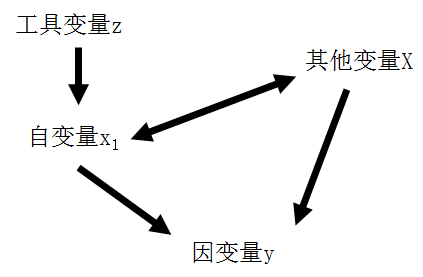
\includegraphics[height=8cm]{tool}
  \caption{工具变量法示意图}
    \label{tool}
\end{figure}

文献\cite{arellano1995another},\cite{nelson1988some},\cite{cragg1993testing}通过数学推导验证了工具变量法的原理和可行性。在文献\cite{陈林2012中国地区性行政垄断与区域经济绩效},\cite{方颖2011寻找制度的工具变量}和\cite{陈昊2014出口贸易与学历误配}中,都利用工具变量法对经济社会体制、经济增长和贸易与学历等社会学问题进行了分析。

\textbf{断点回归方法(regression discontinuity design)}是一种拟随机实验,在进行因果分析时,其分析效果仅次于随机实验的一种方法,能够有效避免因果分析的内生性问题\cite{余静文2011新}。断点回归可以分为两类,一类是模糊断点回归(Fuzzy RD),可以分析协变量是确定型、不连续的情况,另一类是清晰断点回归(Sharp RD),可以分析协变量是概率函数的情况\cite{imbens2008regression}。在利用断点回归模型进行因果检验时,往往还需要对检验结果进行稳健性检验,以验证检验结果的正确性。

该方法是由Thistlethwaite和Campbell在1960年首次提出\cite{thistlethwaite1960regression},在他们的研究中分析了学术获得荣誉奖励与学术成就之间的因果关系。由于学生是否能够获得奖励取决于其考试分数$x$是否能够超过阈值$c$,如果高于阈值则授予奖励,否则不授予。因此在考试成绩$c$出就产生了中断,$c$就是这个断点。当通过分析发现学生的学术成就也发生了类似中断,例如成绩在$c$以下的学生的学术成就低于成绩在$c$以上的学生,那么就可以任务两者之间存在某种因果关系。如图~\ref{score}所示,$x$轴表示学习成绩,其在$c$处的中断对应了$y$轴学术成就的中断,因此可以看出,通过控制考试成绩就可以使得自变量是否取得荣誉奖励与因变量学生的学术成就完全独立,从而可以分析二者之间的因果关系。

\begin{figure}[h] 
  \centering
  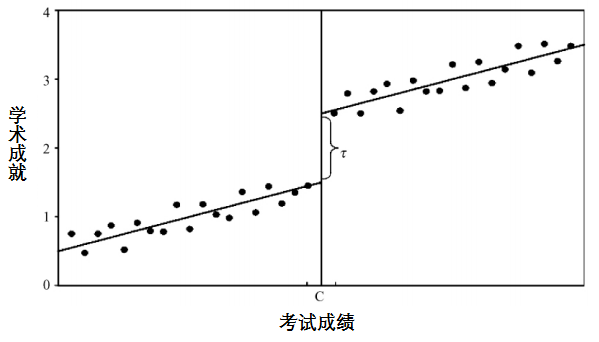
\includegraphics[height=8cm]{score}
  \caption{断点回归方法示意图\cite{lee2010regression}}
  \label{score}
\end{figure}

王骏等人在文献\cite{王骏2015重点高中能否提高学生的学业成绩}中分析了在重点高中就读对学生学习成绩的影响。分析结果表明在重点高中读书对学生的学习成绩仅有轻微的正面影响,对于理科生来说高考成绩优于普通高中,但数值差异不大。而对于文科生来说在两种高中就读的成绩差异并不明显。

张川川等人在文献\cite{zhang2012结婚年龄与婚姻的稳定性}中分析了结婚年龄与婚姻稳定性之间的关系。通过断点回归方法,分析出婚年龄越大,离婚的概率越高的关联关系。而当利用传统最小二乘法进行估计时,结果显示没有明确的因果关系,这表明该方法的分析结果可能存在误差。

张建同等人在文献\cite{张建同2015上海市房地产限购限贷政策评估}对上海市房地产价格指数和地方财政收入月度数据进行分析,研究了上海市房地产限购限贷政策同这两项指标之间的因果关系。分析结果表明该限购措施对房屋的销售价格具有统计意义上的负面影响,但经济意义上并不明显;同时,对地方财政收入产生并没有显著影响。

席鹏辉等人在文献\cite{席鹏辉2015空气污染对地方环保投入的影响}中利用多断点回归模型检验空气污染对地方环保投入的影响。分析结果显示较轻的空气污染会造成环保支出的减少,而当空气污染水平较重时,就不会出现这种情况,二者之间不存在必然联系。


\textbf{格兰杰因果关系检验(Granger Causal Relation Test)}是著名经济学家Clive W. J. Granger提出的一种分析变量之间格兰杰因果关系的的方法,而这种关系是指“依赖于使用过去某些时点上所有信息的最佳最小二乘预测的方差”\cite{格}。即在平稳的时间序列下,对于两个变量$X,Y$,如果利用$X$和$Y$的过去信息对$Y$进行预测时,预测效果要由于单独利用$Y$的过去信息进行预测,则成$X$是$Y$的格兰杰原因\cite{格}。对于格兰杰因果关系来说,其本质是统计意义上的一种因果性,并非实际意义上存在的客观关系,但虽然如此,通过格兰杰因果关系仍然能够揭示两个变量之间的关系。

Hiemstra等人在文献\cite{hiemstra1994testing}中利用线性和非线性格兰杰因果关系检验每日道琼斯股票收益与纽约证券交易所交易量百分比变化之间的动态关系,从中能够发现股票收益与成交量之间存在着显著的双向非线性因果关系。 

游和远等人在文献\cite{游和远2007基于格兰杰因果关系检验模型的地价与房价关系分析}中同样利用格兰杰因果分析方法分析了地价变动与房价变动之间的因果关系,并通过对深圳市真实地价变动与房价变动分析,发现其中并不存在因果关系,否定了人们普遍存在的认为二者之间存在关联的直觉感受。

Haoyen Yang等人在文献\cite{yang2000note}中通过使用1954至1997年期间更新的台湾数据,重新分析了能源消费与GDP之间的因果关系。还分析了台湾国内生产总值与总量之间的因果关系,利用格兰杰因果分析方法,作者还发现总能耗与GDP之间存在双向因果关系。 

Soytas等人在文献\cite{soytas2003energy}中研究了能源消耗与国内生产总值的时间序列特征,并对世界前十大新兴市场重新进行了检验。通过格兰杰因果分析发现能源消耗与GDP在阿根廷成双向因果关系,而在意大利和韩国能源消耗受GDP影响,在土耳其,法国,德国和日本则恰恰相反,即GDP受能源消耗的影响。

虽然格兰杰因果检验的检验效果及其应用方法存在一定争议\cite{庞皓1999格兰杰因果检验的有效性及其应用},\cite{孔凡文2010格兰杰因果关系检验模型分析与应用},但利用其进行因果分析仍然起到一定的启示作用,揭示变量之间存在的一定关系。

\section{基于倾向值匹配的因果分析}

倾向值(propensity score)一词是由Rosenbaum和Rubin在1983年最早提出\cite{rosenbaum1983central},提出这一概念的主要目的还是为了为了排除混淆变量(confounding variables)对因变量的干扰,解决因果分析中的变量内生性的问题。倾向值的本质是一种条件概率,是在混淆变量被控制的条件下,研究因变量受自变量影响的一种条件概率。对于一些问题来说,是没办法利用随机试验来进行因果分析的。例如要研究大学教育对收入的影响,就无法随机找到被试,让一部分上大学而另一部分不是大学对其进行判断。因此为了排除性别、年龄、地域差异等混淆变量对收入的影响,只观察是否上过大学这一条件,就需要通过倾向值匹配的方法来控制或消除这些差异的干扰。

简单来说,倾向值匹配的核心思想就是通过Logistic回归模型或Probit模型将所有混淆变量纳入模型当中,来计算因变量受到自变量影响的概率值,这个概率即为倾向值。然后将所有被试个体分为采用和没采用自变量的两组,对其中所有样本分别计算其倾向值,根据计算得到的倾向值的大小,对两组内的样本进行匹配,倾向值近似的样本匹配成为一对。这样匹配成功的两个样本,其倾向值近似,意味着各种混淆变量的近似相同,而唯一不同的就是是否采用了自变量。因此就可以通过倾向值近似样本的对比来观察自变量对因变量的影响结果\cite{胡安宁2012倾向值匹配与因果推论}。

倾向值匹配算法一经提出,在经济学领域就引起了高度的重视,众多研究开始采用这个方法。

周振等人在文献\cite{周振2014户籍歧视与城乡劳动力工资差异}中分析户籍差别对劳动力工资的影响,将户籍、性别、年龄、教育年限、职业性质、单位类型等因素作为混淆变量,利用倾向值匹配分析其中的因果关系。表~\ref{倾向}显示了利用Logistic回归模型计算的各个样本的倾向值,表~\ref{匹配}显示了对相近倾向值进行匹配之后的结果。

\begin{table}[h]
  \centering
  \caption{城镇居民和务工农民的倾向值} 
  \label{倾向}
  \begin{tabular}{|c|c|c|c|c|c|c|}\hline
  \multirow{2}*{组别}&\multicolumn{3}{c|}{城镇居民}&\multicolumn{3}{c|}{务工农民}\\\cline{2-7}
    & 均值 & 最大值 & 最小值& 均值 & 最大值 & 最小值 \\ \hline
  1 & 0.437721 & 0.607368 & 0.062054 & 0.183598 & 0.272155 &0.020464 \\ 
  2 & 0.723871 &0.811386 & 0.60783 & 0.336588 & 0.395526 & 0.272155\\ 
  3 & 0.870943 & 0.923928 & 0.811634 & 0.462265 & 0.530409  &0.395977\\ 
  4 & 0.941486 & 0.963302 & 0.913953 & 0.607857 & 0.70278  &0.530694\\ 
  5 & 0.977176 & 0.996481 & 0.963386 & 0.82286 & 0.989905  &0.704851\\ 
  total & 0.790239 & 0.996481 & 0.062054 & 0.482652 & 0.989905 & 0.020464\\\hline
  \end{tabular}
\end{table}

\begin{table}[h]
  \centering
  \caption{倾向值匹配结果} 
  \label{匹配}
  \begin{tabular}{|c|c|c|c|c|}\hline
   匹配半径 & 样本 & 城镇居民工资 & 务工农民工资&工资差别 \\ \hline
 & unmatched & 31059.23 & 20438.69 & 10620.54 \\ \hline
  & ATT & 29398.23 &22381.91 & 7016.32\\ 
  $\varepsilon$=0.001& ATU & 20819.65 &24493.87 & 3674.22\\ 
  & ATE &  & & 5892.70\\ \hline
  & ATT & 28056.43 &21803.06 & 6253.37\\ 
  $\varepsilon$=0.0001& ATU & 20525.62 &25543.25 & 5017.63\\ 
  & ATE &  & & 5710.42\\ \hline
  & ATT & 26822.60 &21699.87 & 5122.71\\ 
  $\varepsilon$=0.00003&ATU & 21077.86&25512.25 & 4434.40\\ 
  & ATE &  & & 4792.32\\ \hline
  \end{tabular}
\end{table}

从表中可以看出,对于不同的实验对象能够计算得到不同的倾向值,而在进行倾向值匹配是,选取不同的匹配半径能够获得不同的匹配结果,这样也就使得工资差别的计算结果不同。但是从结果能够看出,倾向值匹配法有效地排除了不相关的混淆变量对工资的影响,分析出户籍与工资之间的因果关系。

侯珂等人在文献\cite{侯珂2014留守对农村儿童青少年社会适应的影响}中分析了父母外出打工对于农村留守儿童在未来压力感知、抑郁、师生关系和幸福感等方面的影响。通过对是否采用倾向值匹配算法分析得到的两种结果进行了对比,验证了倾向值匹配对于因果分析的重要性。

张紫薇等人在文献\cite{张紫薇2016大学本土留学教育个人收益的计量分析}中通过对毕业生调查数据,分析了本土留学教育对个人经济收入的影响。利用倾向值匹配算法排除了个人性别、专业意向、家庭背景等因素对结果的影响,得出了学本土留学教育存在显著经济收益的结论。

Jalan等人在文献\cite{jalan2003estimating}中研究了阿根廷福利计划中与工人收入净增长之间的关系。通过利用倾向值匹配算法,排除了其他因素的异质性影响,发现福利计划的参与者的平均收益增长是总工资的一半以上。同时还验证了该算法的鲁棒性。

Seeger等人在文献\cite{seeger2005application}中利用大量数据资料,分析了他汀类药物治疗对心肌梗死造成的影响,通过使用倾向值匹配算法滤除了许多这种关联的潜在混杂因素,分组归类了他汀类药物的引发剂组和非引发剂组,揭示了其余心肌梗死之间的因果关系。

\section{本章小结}

本章主要对社交网络上的影视剧预测和推荐进行了介绍,由于社交网络的用户群体庞大,产生的数据量也随之增大,利用大数据能够准确地挖掘其中隐含的内在联系,从而对影视剧的宣传推广进行指导。而对于影视剧来说,其所特有的营销需求就是要求广大的受众群体和频繁的曝光度,社交网络正好满足了这一需求,通过在社交网络上的宣传,能够使更多的用户接收到宣传信息,并且引导用户自发扩散信息,实现病毒式传播,病毒式营销。

但是目前现有的各种推广手段所能获得的推广效果不尽相同,对于不同类型的影视剧,不同的宣传方,不同的受众群体,不同的推广手段就会导致不同的推广效果。那么为了能够挖掘出其中的内在联系,寻找最优的推广手段,就需要通过因果分析法,判断推广手段与推广效果之间的因果关系。目前应用比较广泛的因果分析方法有很多种,各自拥有不同的应用场景和分析特性,本章对其中的三种因果分析方法进行了简要介绍。但是可以看出,目前因果分析的各种方法还主要是应用在经济学、社会学等人文社科领域,应用的数据量较小,在计算机科学领域应用较少,尤其是社交网络、影视剧分析等方面更是少有人涉足。

本文选取了其中一种因果分析方法:倾向值匹配法对电视剧的推广模式进行分析。该方法相对于其他因果分析方法来说,能够将研究对象相关的各种变量因素包含到分析过程当中,避免了利用工具变量方法时需要寻找与其他变量完全无关的工具变量的过程,而且有时候这个变量是无法找到的;也避免了利用断点回归方法时用来区分实验组和对照组的断点的寻找。因此,倾向值匹配算法能够获得更广泛的适用性,得到更加严谨的分析结果。




























































